% !TEX root = my-thesis.tex
%
\chapter{Preliminaries}
\label{sec:preliminaries}

To start with, we provide an overview of the key concepts and methods 
our approach relies on. 
First, we discuss the causal knowledge graph CauseNet~\cite{Heindorf2020Causenet} in more detail. 
Next, we examine different types of causal 
questions and discuss the process of curating our causal question dataset. 
Finally, we provide a brief introduction to reinforcement learning, 
including the REINFORCE~\cite{Williams1992REINFORCE} and Synchronous Advantage Actor-Critic (A2C)~\cite{Mnih2016A2C} algorithms.

\section{CauseNet}
\label{subsec:causal-kgs}
CauseNet~\cite{Heindorf2020Causenet} is a large-scale causal knowledge graph of causal relations.
Specifically, CauseNet contains \textit{claimed} causal relations because they were extracted 
from web sources like Wikipedia and ClueWeb12\footnote{\url{https://lemurproject.org/clueweb12/}} that are not necessarily true.
Formally, CauseNet is defined as $\mathcal{K} = (\mathcal{E}, \mathcal{R})$, where 
$\mathcal{E}$ represents the set of entities and $\mathcal{R}$ is the set of relations. 
The entities in CauseNet are single words or noun phrases, while the set of relations 
contains only the \textit{mayCause} relation, i.e., $\mathcal{R} = \{mayCause\}$.\footnote{In this thesis we will use \textit{cause} when talking about the relations.}
Figure~\ref{fig:graph_example} shows an excerpt from CauseNet. It shows the entity \textit{pneumonia} together 
with some of its causes and effects. The causal relations are stored as triples, e.g., 
$(pneumonia, mayCause, sepsis) \in \mathcal{K}$ where $pneumonia, sepsis \in \mathcal{E}$.
Moreover, CauseNet contains additional meta-information for each relation.
Included are the original source, i.e., the URL of the web page and the original sentence,
if applicable.

%The causal relations were extracted from Wikipedia and 
%First, they defined a set of established causal relations containing a cause and an effect, e.g., 
%\textit{smoking} and \textit{cancer}.
%Next, they searched for sentences that contain the cause and effect of one relation and extracted linguistic patterns from the sentences.
%Consequently, the linguistic pattern can be used to find further causal relations.
CauseNet has two configurations, a high-precision one (CauseNet-Precision) and a high-recall one (CauseNet-Full).
The statistics of both graphs can be seen in Table~\ref{table-causenet}.
%CauseNet-Full contains all extracted relations, while CauseNet-Precision
%only contains relations that were extracted by patterns
%which received a support of atleast two. Heindorf et al.~\cite{Heindorf2020Causenet} defined the support of a pattern by the number of seeds 
%which made use of the pattern.
CauseNet-Precision contains around 2\% of the original relations, increasing 
the precision from 83\% to 96\%. The precision was evaluated by randomly selecting 
a number of relations from the graphs and manually evaluating them for correctness.

\begin{table}
\caption{The statistics of CauseNet-Full and CauseNet-Precision, including their precision,
the number of entities, and the number of relations. The numbers were taken from the paper~\cite{Heindorf2020Causenet}.}
\label{table-causenet}
\centering
\begin{tabular}{lrrr} 
			\toprule
			\textbf{Graph} & \textbf{Precision} & \textbf{|Concepts/Entities|} & \textbf{|Relations|}\\
			\toprule
		   CauseNet-Full & 83\% & 12,186,31& 11,609,89 \\
		   CauseNet-Precision & 96\% & 80,223 &	197,806\\
			\bottomrule
\end{tabular}
\end{table}

\section{Causal Questions}
\label{subsec:causal-questions}

Causal questions seek to determine whether there exists a causal relationship 
between different events or phenomena. Often, their goal is to understand why something 
happened or to predict what kind of effects a certain cause might have in the future.

Generally, we can differentiate between different types of causal questions.
Starting with simple binary questions that ask for the validity of a 
causal relation, such as \textit{``Does smoking cause cancer?''}. Another type are 
Cause-Effect questions which seek to identify the cause of a given effect or vice versa.
An example of this type of question is \textit{``What causes the rise in global temperatures?''}.
Additionally, there are more complex questions that investigate the relationship between multiple entities.
For example, a question like \textit{``How does smoking cause cancer?''} examines the specific mechanisms by which the cause produces the effect.
For the first version of our approach, we only consider binary causal questions like 
many prior approaches~\cite{HassanzadeshCausalQA2019, KayeshCausalTransfer2020}.
However, we discuss a simple extension to Cause-Effect questions in Chapter~\ref{ch:discussion}
for future work.

To construct a dataset of binary causal questions, we extracted them from the Webis-CausalQA-22 corpus~\cite{Bondarenko2022CausalQA}.\footnote{\url{https://zenodo.org/record/7476615}}
CausalQA is a corpus for causal question answering containing around 1.1 million
causal questions. The corpus was constructed by extracting causal questions from ten
well-known question answering datasets, such as SQuAD v2.0~\cite{rajpurkar:2018} and MS MARCO~\cite{nguyen:2016}.
For a full list of the datasets, including their references, see Table~\ref{table-causal-datasets}.
The table also shows the number of total causal questions and the number of binary 
causal questions that we extracted for each dataset. After the extraction, only
MS MARCO contains a sufficient number of binary causal questions for use in our experiments.
The scarcity of binary causal questions in the datasets may be due to a number of reasons. One factor is that many datasets, 
such as NewsQA~\cite{trischler:2017} and HotpotQA~\cite{yang:2018}, have a limited number of causal questions to begin with.
Additionally, some larger datasets like ELI5~\cite{fan:2019} are focused on open-ended question
 answering.


\begin{table}
\caption{A few binary causal questions that we extracted from the datasets. The 
cause of each question is colored in \textcolor{tab20darkgreen}{green}, and the effect in \textcolor{tab20darkblue}{blue}.}
\label{table-example-questions}
	\centering
\begin{tabular}{lc}
	\toprule
	\textbf{Question} & \textbf{Answer}\\
	\midrule
	Can \textcolor{tab20darkgreen}{alcohol} cause \textcolor{tab20darkblue}{diabetes}? & Yes \\
	Will \textcolor{tab20darkgreen}{hot weather} affect \textcolor{tab20darkblue}{blood sugar}? & Yes \\
	Is \textcolor{tab20darkblue}{malaria} caused by a \textcolor{tab20darkgreen}{fungus}? & No \\
	Does \textcolor{tab20darkgreen}{depo provera} cause \textcolor{tab20darkblue}{cancer}? & No \\
	\bottomrule
\end{tabular}
\end{table}

\newcommand{\pattern}[1]{\texttt{\fontsize{9.5pt}{10pt}\selectfont [#1]}\xspace}
For the extraction of binary causal questions, we built on work by 
Heindorf et al.~\cite{Heindorf2020Causenet} from CauseNet.
For their evaluation, they implemented an extraction mechanism for binary causal questions.
Specifically, the questions were extracted via patterns of the following form:
\begin{center}
\texttt{\selectfont [question word]\xspace}
\texttt{\selectfont [cause/effect]\xspace}
\texttt{\selectfont [causal cue word]\xspace}
\texttt{\selectfont [cause/effect]\xspace} ?
\end{center}
where the \texttt{\selectfont [question word]\xspace} placeholder either represents one of the question words from 
Table~\ref{table-questions-pos-tags} or is empty. The \texttt{\selectfont [causal cue word]\xspace} placeholder 
represents words that are good indicators for causal relations together with their appropriate prepositions. Therefore, they should 
identify whether a question is causal or not. The original approach
only considered \textit{cause} in different verb forms, e.g., infinitive, past, or progressive.
We extended this to consider a greater number of causal cue words.
Specifically, we used the collection from Girju et al.~\cite{Girju2002CausalCue}.
Girju et al. curated a collection of causal cue words and ranked them by their 
frequency and ambiguity, i.e., how often they appear in text and how often they 
refer to a causal relation. 
Among these, we selected the ones that were ranked with high frequency and low 
ambiguity.
Table~\ref{table-cue-words} shows the full list of 23 words. 

Moreover, the \texttt{\selectfont [cause/effect]\xspace} placeholder 
represents causal concepts, where one takes the role of the cause and the other 
the role of the effect. The order depends on the question word and the causal cue word. Like
 Heindorf et al.~\cite{Heindorf2020Causenet}, we place a few restrictions 
on the questions to keep the causal concepts simpler. This should increase 
the probability that the concepts can be found in CauseNet because we can only 
use questions where both the cause and effect can be found. The restrictions are 
enforced by filtering questions on a number of POS-Tags from the Stanford CoreNLP~\cite{Manning2014NLP}.
The full list is shown in Table~\ref{table-questions-pos-tags} on the right.
Among others, we disallow coordinating conjunctions or subordinating conjunctions.
Finally, we check whether the questions are answered with ``yes'' or ``no'' and remove 
any further explanation. Table~\ref{table-example-questions} shows a few questions which 
we extracted from the datasets.

To summarize, the extraction focuses on binary causal questions that contain 
exactly one cause and one effect identified by one of 23 causal cue words.

%\begin{table}
\centering
\caption{The ten datasets that are part of CausalQA~\cite{Bondarenko2022CausalQA}. The
		\textit{Total} column shows the total number of causal questions for each dataset, 
		while the \textit{Binary} column shows the number of binary causal questions.
		Note that the test sets are either not publically available or 
		are missing the answers.}
\label{table-causal-datasets}
	\begin{tabular}{lrrrrr} 
		\toprule
		\textbf{Dataset} & \multicolumn{2}{c}{\textbf{Total}} & \multicolumn{2}{c}{\textbf{Binary}} & \textbf{Reference} \\
		\cmidrule(lr{.6em}){2-3} \cmidrule(l{0.4em}){4-5}
		&\textbf{|Train|} & \textbf{|Valid|} & \textbf{|Train|} & \textbf{|Valid|} & \\
		\midrule
		PAQ & 692,645 & 76,961 & 1 & --  & \cite{Lewis2021PAQ}\\ 
		GooAQ & 146,253 & 33 & 167 & -- &  \cite{khashabi:2021}\\
		MS MARCO & 41,764 & 2,558 & 2,410 & 263 & \cite{nguyen:2016} \\
		Natural Questions & 2,796 & 71 & -- & -- & \cite{kwiatkowski:2019}\\
		ELI5 & 131,035 & 4,834 & 2 & --  & \cite{fan:2019}\\
		SearchQA &663 & 117 & -- & -- & \cite{dunn:2017}\\
		SQuAD v2.0 & 4,342 & 483 & -- & -- & \cite{rajpurkar:2018}\\
		NewsQA &1,303 & 62 & -- & -- & \cite{trischler:2017}\\
		HotpotQA &355& 35 & -- & -- & \cite{yang:2018}\\
		TriviaQA & 637 & 66 & -- & -- & \cite{joshi:2017} \\
		\bottomrule
	\end{tabular}
\end{table}
\begin{table}
\caption{The causal cue words we used to detect binary causal questions. The list was
		curated by Girju et al.~\cite{Girju2002CausalCue} to include words that are 
		good indicators for causal relations, meaning they should have low ambiguity and high frequency.}
\label{table-cue-words}
\centering
	\begin{tabular}{rrrr}
	\toprule
	\multicolumn{4}{c}{\textbf{Causal Cue Words}} \\
	\midrule
	induce & provoke & relate (to) & trigger off \\
	give rise (to) & arouse & link (to) & bring on \\
	produce & elicit & stem (from)& result (from)\\
	generate & lead (to)& originate & trigger\\
	effect & derive (from)& bring forth& cause \\
	bring about & associate (with)& lead up &\\
	\bottomrule
	\end{tabular}
\end{table}
\begin{table}
\caption{The left table shows the question words we used for the binary question
extraction. The right table shows the forbidden POS tags for the binary question extraction.}
\label{table-questions-pos-tags}
	\centering
	\begin{tabular}{rr}
		\toprule
		\multicolumn{2}{c}{\textbf{Question Words}} \\
		\midrule
		is & do\\
		can  & does\\
		might & did \\
		would & will \\
		could & are\\
		may \\
		\bottomrule
	\end{tabular}
	\quad
	\begin{tabular}{ll}
		\toprule
		\textbf{POS-Tag} & \textbf{Description}\\
		\midrule
		CC & Coordinating conjunction \\
		IN & Preposition or subordinating conjunction \\
		TO & To-prepositions \\
		WDT & Wh-determiner \\
		WP & Wh-pronoun \\
		WRB & Wh-adverb \\
		\bottomrule
	\end{tabular}
\end{table}
\begin{table}
\centering
\caption{The ten datasets that are part of CausalQA~\cite{Bondarenko2022CausalQA}. The
		\textit{Total} column shows the total number of causal questions for each dataset, 
		while the \textit{Binary} column shows the number of binary causal questions.
		Note that the test sets are either not publically available or 
		are missing the answers.}
\label{table-causal-datasets}
	\begin{tabular}{lrrrrr} 
		\toprule
		\textbf{Dataset} & \multicolumn{2}{c}{\textbf{Total}} & \multicolumn{2}{c}{\textbf{Binary}} & \textbf{Reference} \\
		\cmidrule(lr{.6em}){2-3} \cmidrule(l{0.4em}){4-5}
		&\textbf{|Train|} & \textbf{|Valid|} & \textbf{|Train|} & \textbf{|Valid|} & \\
		\midrule
		PAQ & 692,645 & 76,961 & 1 & --  & \cite{Lewis2021PAQ}\\ 
		GooAQ & 146,253 & 33 & 167 & -- &  \cite{khashabi:2021}\\
		MS MARCO & 41,764 & 2,558 & 2,410 & 263 & \cite{nguyen:2016} \\
		Natural Questions & 2,796 & 71 & -- & -- & \cite{kwiatkowski:2019}\\
		ELI5 & 131,035 & 4,834 & 2 & --  & \cite{fan:2019}\\
		SearchQA &663 & 117 & -- & -- & \cite{dunn:2017}\\
		SQuAD v2.0 & 4,342 & 483 & -- & -- & \cite{rajpurkar:2018}\\
		NewsQA &1,303 & 62 & -- & -- & \cite{trischler:2017}\\
		HotpotQA &355& 35 & -- & -- & \cite{yang:2018}\\
		TriviaQA & 637 & 66 & -- & -- & \cite{joshi:2017} \\
		\bottomrule
	\end{tabular}
\end{table}
\begin{table}
\caption{The left table shows the question words we used for the binary question
extraction. The right table shows the forbidden POS tags for the binary question extraction.}
\label{table-questions-pos-tags}
	\centering
	\begin{tabular}{rr}
		\toprule
		\multicolumn{2}{c}{\textbf{Question Words}} \\
		\midrule
		is & do\\
		can  & does\\
		might & did \\
		would & will \\
		could & are\\
		may \\
		\bottomrule
	\end{tabular}
	\quad
	\begin{tabular}{ll}
		\toprule
		\textbf{POS-Tag} & \textbf{Description}\\
		\midrule
		CC & Coordinating conjunction \\
		IN & Preposition or subordinating conjunction \\
		TO & To-prepositions \\
		WDT & Wh-determiner \\
		WP & Wh-pronoun \\
		WRB & Wh-adverb \\
		\bottomrule
	\end{tabular}
\end{table}
\begin{table}
\caption{The causal cue words we used to detect binary causal questions. The list was
		curated by Girju et al.~\cite{Girju2002CausalCue} to include words that are 
		good indicators for causal relations, meaning they should have low ambiguity and high frequency.}
\label{table-cue-words}
\centering
	\begin{tabular}{rrrr}
	\toprule
	\multicolumn{4}{c}{\textbf{Causal Cue Words}} \\
	\midrule
	induce & provoke & relate (to) & trigger off \\
	give rise (to) & arouse & link (to) & bring on \\
	produce & elicit & stem (from)& result (from)\\
	generate & lead (to)& originate & trigger\\
	effect & derive (from)& bring forth& cause \\
	bring about & associate (with)& lead up &\\
	\bottomrule
	\end{tabular}
\end{table}



\section{Reinforcement Learning}
\label{subsec:rl}
In the following, we introduce some preliminaries regarding reinforcement learning,
including the REINFORCE~\cite{Williams1992REINFORCE} and Synchronous Advantage Actor-Critic (A2C)~\cite{Mnih2016A2C} algorithms.
As done by related work~\cite{Xiong2017DeePpath, Das2018Minerva, Kaiser2021Reinforcement}, we focused on policy gradient methods~\cite{Sutton1998RL} because 
they can better deal with the large action space in knowledge graphs compared to value function-based methods~\cite{Xiong2017DeePpath}.

In the reinforcement learning setting, an agent interacts with an environment to maximize a reward 
depending on some specified goal, e.g., moving a robot~\cite{Peng2018Mimic}.
Formally, we define a Markov Decision Process (MDP)~\cite{Sutton1998RL} as a 4-tuple 
$(\mathcal{S}, \mathcal{A}, \delta, \mathcal{R})$. The MDP consists of the state space $\mathcal{S}$,
 the action space $\mathcal{A}$, the transition function $\delta : \mathcal{S} \times 
 \mathcal{A} \rightarrow \mathcal{S}$, and the reward function 
 $\mathcal{R} : \mathcal{S} \rightarrow \mathbb{R}$.
When selecting an action $a_t$ in state $s_t$, the environment changes from state $s_t$ to the next state $s_{t+1}$ 
via the transition function, i.e., $\delta(s_t, a_t) = s_{t+1}$. 
Generally, the transition function can be probabilistic or deterministic. In this thesis, we consider 
deterministic transition functions because the graph is static and completely defines the transition function~\cite{Shen2018MWalk}. 
Therefore, for each action $a_t$ in state $s_t$, the next state $s_{t+1}$ is known.
Additionally, the environment gives a reward $\mathcal{R}(s_{t+1}) = r_t$ at each time step $t$.

The agent is represented by a policy network $\pi_{\theta}(a_t | s_t)$ parametrized by $\theta$.
The policy network computes a probability distribution over actions $a_t$ at state $s_t$ at each time step $t$.

Figure~\ref{fig:rl} demonstrates the interaction between the agent and the environment:
\begin{enumerate}
	\item In state $s_t$, the agent selects an action $a_t$ via the policy network and applies the action to the environment.
	\item The environment evolves via $\delta(s_t, a_t)$ to $s_{t+1}$ and gives a scalar reward $r_{t+1}$.
	\item The agent receives state $s_{t+1}$ and reward $r_{t+1}$, and the next iteration starts.
\end{enumerate}
The process is continued until the maximum number of steps $T$ is reached, or the agent reaches a terminal state, e.g., the end of a game.

Overall, the agent is supposed to maximize the expected return~\cite{Schulman2016GAE, Peng2018Mimic}:
\begin{equation}
	J (\theta) = \mathbb{E}_{\pi_\theta} \left[ \sum_{t=0}^T \gamma^t \, r_t\right] 
\end{equation}
where $r_t$ are the rewards from the environment for each time step $t$ and the expectation is taken over episodes 
sampled from the current policy $\pi_\theta(a_t | s_t)$. The parameter $\gamma$ is the discount factor between 0 and 1, which is used to 
weigh rewards from later time steps less.
In the general setting, the episode length $T$ can be infinite. However, we only consider finite episodes up to a maximum length of $T$ as 
described in Section~\ref{sec:approach-description}.\footnote{In the infinite setting, the discount factor $\gamma$ is also used to keep the expected return finite~\cite{Peng2018Mimic}.}

For many different policy gradient methods, the expected return is optimized via the following gradient~\cite{Schulman2016GAE}:
\begin{equation}
	\nabla_{\theta} J (\theta) = \mathbb{E}_{\pi_\theta} \left[ \sum_{t=0}^T \nabla_\theta \, \log(\pi_\theta (a_t | s_t)) \Psi_t \right] 
	\label{eq:polupdate}
\end{equation}

\begin{figure}
	\centering
	%\hspace{-3cm}
	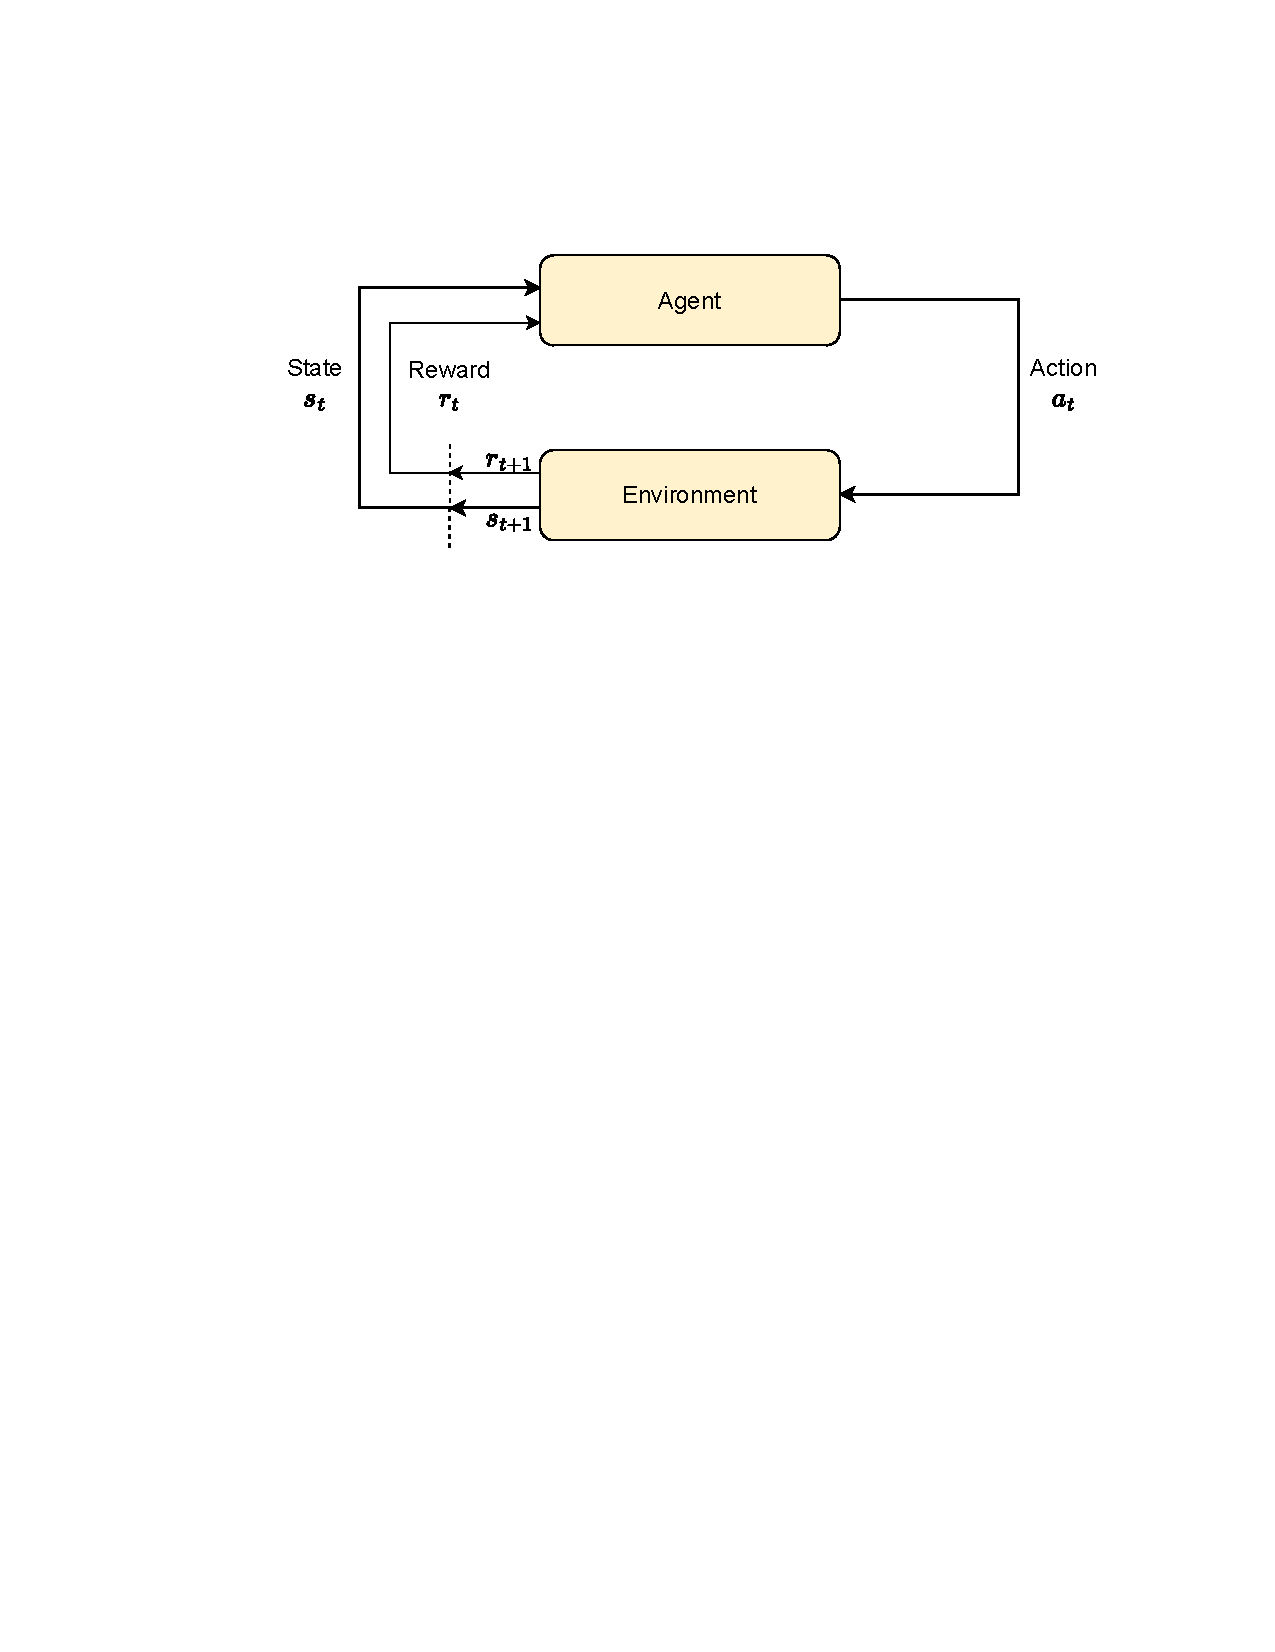
\includegraphics[clip, trim=3cm 18cm 3cm 3cm, width=1.0\textwidth]{figures/rl}
	\caption{The figure shows the general reinforcement learning setting, where an agent interacts with an environment. The agent applies an action on the environment at each time step 
	and receives the next state and a reward. The figure was taken from Sutton et al.~\cite{Sutton1998RL}.}
	\label{fig:rl}
\end{figure}

where $\Psi_t$ is a value estimating the returns or advantages as described below, and the expectation is again 
taken over episodes sampled from the current policy $\pi_\theta(a_t | s_t)$. As usual, the gradient 
steps are done in batches of episodes via gradient descent, as shown in Section~\ref{sec:approach-description}. 

The value $\Psi_t$ can take several forms~\cite{Schulman2016GAE}. In the following, we 
introduce three of them, the Monte-Carlo return, the advantage, and GAE~\cite{Schulman2016GAE}.

\paragraph{Monte-Carlo Return}

The first option is the Monte-Carlo return~\cite{Schulman2016GAE, Peng2018Mimic}, also called the reward to go. The Monte-Carlo return computes the sum of rewards from 
step $t$ onwards and is defined as: 
\begin{equation}
	R_t = \sum_{i=0}^{T-t} \gamma^{i} \, r_{t+i}
	\label{eq:return}
\end{equation}
where $r_t$ are the rewards from the environment at each time step $t$ and $\gamma$ is the discount factor.
Setting $\Psi_t = R_t$ yields the REINFORCE~\cite{Williams1992REINFORCE} algorithm.
In this setup, $R_t$ determines the direction of the gradient update in Equation~\ref{eq:polupdate}. It should increase the probability 
of actions $a_t$ that lead to positive rewards and decrease the probability of actions leading to negative rewards.

However, while the Monte-Carlo return is an unbiased estimate of the expected return, it has a very high variance because each reward $r_t$ is a random variable that depends on randomness 
coming from the policy network $\pi_{\theta}(a_t | s_t)$~\cite{Peng2018Mimic}.\footnote{In case of probabilistic transition functions, there is also additional randomness coming from the environment.}
One possibility to reduce the variance while keeping the estimate unbiased is the substraction of a baseline $b_t$, such that $\Psi_t = R_t - b_t$~\cite{Mnih2016A2C}.
For example, $b_t$ could be a moving average of the Monte-Carlo return~\cite{Das2018Minerva}.


\paragraph{Advantage}
Another option to decrease the variance of the estimate is the introduction of a critic~\cite{Sutton1998RL}. In the resulting 
Actor-Critic setting, we have our policy network $\pi_\theta(a_t | s_t)$ representing the actor and a value network $V_\psi(s_t)$ parametrized by $\psi$ representing the critic.
The value network $V_\psi(s_t)$ should predict the value of the state $s_t$. In the 
Synchronous Advantage Actor-Critic (A2C) algorithm~\cite{Mnih2016A2C}, the value network is trained to predict the 
Monte-Carlo return $R_t$ from Equation~\ref{eq:return}. Subsequently, the advantage is defined as:
\begin{equation}
	\mathcal{A}_t^\psi = R_t - V_\psi(s_t)
	\label{eq:advantage}
\end{equation}
A2C then sets $\Psi_t = \mathcal{A}_t^\psi$ and uses Equation~\ref{eq:polupdate} to update the policy network.
In this case, the advantage $\mathcal{A}_t$ determines the direction of the gradient update. It increases or decreases the 
probability of actions $a_t$ depending on whether they are better or worse than average~\cite{Schulman2016GAE}.
Simultaneously, the value network is updated via the mean-squared error between the predictions 
of the value network $V_\psi(s_t)$ and the Monte-Carlo return $R_t$.

\paragraph{Generalized Advantage Estimation (GAE)}
Alternatively, we can replace the advantage in the policy network update with the 
generalized advantage estimate (GAE)~\cite{Schulman2016GAE} to further reduce the variance and achieve more control over the trade-off between bias and variance. Similarly, we can replace the Monte-Carlo return in the value network 
update with the $\lambda$-return~\cite{Sutton1998RL}.
In the following, we introduce the GAE and $\lambda$-return following the 
explanation from Peng et al.~\cite{Peng2018Mimic}.

Until now, the expected return is estimated via the unbiased Monte-Carlo 
return (Equation~\ref{eq:return}).
As discussed above, this estimator has a very high variance.
To address this problem, we can introduce $n$-step returns to decrease the variance.
The $n$-step return does not compute the complete sum until time step $T$ like the Monte-Carlo
return. Instead, the sum is computed for $n$ steps, and after that point, the estimate is 
bootstrapped via the value network $V_\psi(s_{t+n})$~\cite{Silver2015RL, Peng2018Mimic}:
\begin{equation}
	R_t^{(n)} = \sum_{i=0}^{n-1} \gamma^i \, r_{t+i} + \gamma^n V_{\psi} (s_{t+n}) 
\end{equation}
The disadvantage is that the bootstrap estimate via the value network introduces some bias.
Hence, the parameter $n$ can be used to control the trade-off between 
bias and variance. Specifically, high $n$ yield a lower bias but higher variance, whereas 
small $n$ yield a higher bias but lower variance. For example, setting $n=\infty$ gives us the 
Monte-Carlo return $R_t$ from Equation~\ref{eq:return}, assuming that all rewards after the maximum 
episode length $T$ are $0$~\cite{Peng2018Mimic}.

However, now arises the question of which $n$ we should choose. We could treat it as 
a hyperparameter and optimize the setting on some validation set.
Instead, the literature introduced the $\lambda$-return~\cite{Sutton1998RL} to deal with this problem.
The $\lambda$-return does not take a specific $n$ but rather computes the exponentially 
weighted average over all of them~\cite{Peng2018Mimic}: 
\begin{equation}
	%\vspace{-1cm}
	R_t(\lambda) \stackrel{(1)}{=} (1- \lambda) \sum_{n=1}^{\infty} \lambda^{n-1} R_t^{(n)} \stackrel{(2)}{=} (1-\lambda) \sum_{n=1}^{T-t-1} \lambda^{n-1} \, R_t^{(n)} + \lambda^{T-t-1} R_t^{(T-t)} 
\end{equation}
where $\lambda$ is a hyperparameter between $0$ and $1$, which can be used to control the trade-off between bias and variance. Equality (1) shows the general
form of the $\lambda$-return up to infinity. Equality (2) holds if all  
rewards after time step $T$ are $0$~\cite{Peng2018Mimic}. For more details, see 
the appendix of Peng et al.~\cite{Peng2018Mimic}.

Finally, we set the advantage in Equation~\ref{eq:advantage} to $\mathcal{A}_t^{\psi} = R_t(\lambda) - V_\psi(s_t)$, 
which corresponds to the GAE~\cite{Schulman2016GAE}.
Moreover, we optimize the value network via the mean-squared error between the predictions of the value network $V_\psi(s_t)$ and the
$\lambda$-returns $R_t(\lambda)$~\cite{Peng2018Mimic}, as shown in Section~\ref{sec:approach-description}.

%\section{Language Models}
%\label{subsec:language-models}


%\paragraph{Notation}

%\begin{itemize}
	%\item entities in the graph $e \in \mathcal{E}$
	%\item question $q$
	%\item question embedding $q_{emb}$
	%\item cause and effect from question $e_c$ and $e_e$
	%\item state $s_t = (q, e_t, h_t)$ or $(q_{emb}, e_{t_{emb}}, h_t)$
	%\item action $a_t = e_{t+1}$
	%\item path rollout $p=((s_0,a_0),(s_1, a_1), \dots, (a_{T_1}, s_{T-1}))$
	%\item mathbf for embeddings
	%\item maybe converter function?
%\end{itemize}






